


\section{Introduction}

A polygon is a closed chain of edges. Several algorithms are available for
polygons. For some of those algorithms, it is necessary that the polygon is
simple. A polygon is simple if edges don't intersect, except consecutive edges,
which intersect in their common vertex.

The following algorithms are available:
\begin{itemize}
\item find the leftmost, rightmost, topmost and bottommost vertex.
\item compute the (signed) area.
\item check if a polygon is simple.
\item check if a polygon is convex.
\item find the orientation (clockwise or counterclockwise)
\item check if a point lies inside a polygon.
\end{itemize}
All those operations take two forward iterators as parameters in order to
describe the polygon. These parameters have a point type as value type.

The type \ccc{Polygon_2} can be used to represent polygons.
Polygons are dynamic. Vertices can be modified, inserted and erased.
They provide the algorithms described above as member functions.
Moreover, they provide ways of iterating over the vertices and edges.

Currently, the \ccc{Polygon_2} class is a nice wrapper around a container of
points, but little more. Especially, computed values are not cached.
That is, when the \ccc{is_simple()} member function is called twice or more,
the result is computed each time anew. 

\section{Example}

The following code fragment creates a polygon and does some checks.

\ccIncludeExampleCode{Polygon/Polygon.cpp}



\begin{figure}
\begin{ccTexOnly}
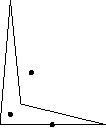
\includegraphics[width=0.5\textwidth]{Polygon/pgn_algos}
\end{ccTexOnly}
\begin{ccHtmlOnly}
<CENTER>
<img border=0 src="./pgn_algos.gif" align=middle alt="Example polygon">
</CENTER>
\end{ccHtmlOnly}
\caption{A polygon and some points
\label{I1_Fig_a_polygon}}
\end{figure}

\ccIncludeExampleCode{Polygon/polygon_algorithms.cpp}
